% ============================================================
%  Experiment 9 --- Project Creation in SCADA (IoT)
%  Sourced from the department's i-Factory IIoT Training Manual,
%  Module 3: Project Creation in SCADA.
% ============================================================
\experimentheader{9}{Experiment 9}{Project Creation in SCADA (IoT)}{IoT Lab}

\begin{objectives}
  \begin{enumerate}
    \item To understand the role and capabilities of SCADA software in an industrial IoT system.
    \item To create a working SCADA project, including a Project Node and a SCADA Node.
    \item To configure a communication link (Comport) between the SCADA node and an automation device.
    \item To select and configure IO Tags and Internal Tags for a chosen subset of the trainer's available sensors.
    \item To configure basic alarms on analog and discrete tags.
    \item To enable ODBC data logging, so tag history becomes available for dashboarding later in this experiment.
    \item To build a WISE-IoTSuite/Dashboard panel that visualises the sensors selected earlier in this experiment.
  \end{enumerate}
\end{objectives}

\begin{equipment}
  \begin{itemize}
    \item PC/laptop with Advantech WebAccess/SCADA installed (Project Node and SCADA Node)
    \item Siemens S7-1200 PLC (or equivalent), with an existing ladder-logic program and known I/O/DB addressing
    \item Ethernet cable and a configured local network connection between the PC and the PLC
    \item TIA Portal (or equivalent Siemens engineering software) for reference to the PLC's tag addresses
    \item WISE-IoTSuite/Dashboard, with a PostgreSQL data source pre-configured by your instructor (host, database, and schema)
  \end{itemize}
\end{equipment}
\newpage

\begin{introduction}
  Supervisory Control and Data Acquisition (SCADA) software sits between the plant floor and the people (or systems) that need to monitor and control it. It collects real-time data from automation devices --- PLCs, controllers, direct digital control (DDC) systems, and distributed control systems (DCS) --- and presents that data through live displays, trends, alarms, and reports.
  \vspace*{1.5em}

  Advantech WebAccess/SCADA, used in this experiment, is a 100\% web-based SCADA package: projects are developed and accessed through a standard web browser, rather than a dedicated desktop client. This lowers the barrier to remote monitoring and multi-site deployment, and it integrates directly with IoT dashboards and cloud platforms via MQTT.
  \vspace*{1.5em}

  A WebAccess/SCADA system is built from three components:
  \begin{itemize}
    \item \textbf{Project Node} --- the development platform and web server. All project configuration, graphics, and database files are stored here, and every client connects to it first.
    \item \textbf{SCADA Node} --- runs the real-time Kernel (\texttt{datacore.exe}), which uses communication drivers to talk to automation hardware (PLCs, I/O modules, controllers) and supplies live data to clients.
    \item \textbf{ViewDAQ Client} --- the browser-based interface used to monitor and control the SCADA node: viewing live graphics, historical trends, and alarms, and adjusting set points.
  \end{itemize}
  In a small setup (as in this lab), the Project Node and SCADA Node commonly run on the same machine.
  \vspace*{1.5em}

  Data inside WebAccess/SCADA is represented as \textbf{Tags}. There are two broad categories:
  \begin{itemize}
    \item \textbf{IO Tags} --- real-time measurements and outputs read from, or written to, an automation device. IO Tags can be Analog (floating-point), Discrete (an integer 0--7, commonly used as a 0/1 digital value), or Text (an ASCII string up to 72 characters).
    \item \textbf{Internal Tags} --- values that exist inside the SCADA software itself rather than being read from a device: \textbf{Constant} tags (a user-defined fixed or operator-editable value), \textbf{Calculation} tags (a mathematical/logical expression over up to 20 other tags), and \textbf{Accumulation} tags (an integration/totaliser over another tag, e.g.\ totalising flow into volume).
  \end{itemize}
  Both tag categories share the same alarm, security, logging, and reporting features once created.
  \vspace*{1.5em}

  The pipeline for this experiment is shown in Figure~\ref{fig:exp9-pipeline}.

  \begin{boxedfigure}
    \centering
    \begin{tikzpicture}[node distance=9mm and 14mm]
      % --- WebAccess group: Project Node above SCADA Node, stacked vertically ---
      \node[block, minimum width=2.8cm] (project) {WebAccess\\Project Node};
      \node[block, below=12mm of project, minimum width=2.8cm] (scada) {SCADA Node};

      % --- Database node, to the left of Project Node ---
      \node[block, left=of project, minimum width=2.4cm, xshift=-5mm] (db) {PostgreSQL};

      % --- PLC node, below SCADA Node ---
      \node[block, below=12mm of scada, minimum width=2.4cm] (plc) {PLC\\(S7-1200)};

      % --- Dashboard node, to the right of Project Node ---
      \node[block, right=of project, minimum width=2.6cm] (dash) {WISE-IoTSuite/\\Dashboard};

      % --- bidirectional arrows, following the vendor's architecture diagram ---
      \draw[arr, <->] (db) -- (project) node[midway, above, font=\small\plexmedium] {ODBC};
      \draw[arr, <->] (project) -- (scada) node[midway, right, font=\small\plexmedium] {RP};
      \draw[arr, <->] (scada) -- (plc);
      \draw[arr, ->] (project) -- (dash);

      % --- dotted boundary around Project Node + SCADA Node, as in the vendor diagram ---
      \begin{scope}[on background layer]
        \node[draw=accentblue, dotted, thick, rounded corners=2pt,
          fit=(project)(scada), inner sep=7mm, label={[accentblue,font=\small\plexmedium]above:WebAccess/SCADA}] (webaccessbox) {};
      \end{scope}
    \end{tikzpicture}
    \captionof{figure}{Data pipeline for this lab experiment.}
    \label{fig:exp9-pipeline}
  \end{boxedfigure}

  \begin{itemize}
    \item The PLC is read either through WebAccess's native Siemens S7 driver (TCP port \texttt{102}) or through an OPC Server (TCP port \texttt{4840}) --- both paths are shown for the sensors used in this experiment (Table~\ref{tab:exp9scada-sensors}).
    \item Each tag has its own \textbf{Log Data} setting (Yes/No), which determines whether that tag's history is recorded at all.
    \item Separately, the \textbf{SCADA Node} has a node-wide \textbf{Data Log to ODBC} setting (\textbf{Edit Node} $\to$ \textbf{Data Log} tab): once enabled, WebAccess periodically writes logged tag values out to an external database via ODBC, at an interval you configure (or by deadband, if the interval is set to \texttt{0}).
    \item In this training's setup, that external database is \textbf{PostgreSQL} (schema \texttt{iot}), and the Dashboard queries a table it refers to as \texttt{data log} to populate panels --- this is why a tag must exist in WebAccess \emph{and} have Data Log enabled \emph{and} have the node's ODBC logging turned on, before it can appear on a dashboard later in this experiment.
  \end{itemize}
\end{introduction}

\begin{boxedtable}
  \captionof{table}{Example Siemens S7-1200 address mapping to WebAccess tag addressing.}
  \label{tab:exp9scada-addrmap}
  {\renewcommand{\arraystretch}{1.5}
    \centering
    \begin{tabular}{llcl}
      \toprule
      Siemens S7-1200 address & Data type & Length (bits) & WebAccess address    \\
      \midrule
      \%I0.4                  & Bool      & 1             & IX000 (start bit 4)  \\
      \%Q0.3                  & Bool      & 1             & QX000 (start bit 3)  \\
      \%M0.4                  & Bool      & 1             & MX000 (start bit 4)  \\
      \%MW0                   & UInt      & 16            & MW000 (start bit 0)  \\
      \%IW6.4                 & UInt      & 16            & IW006 (start bit 4)  \\
      \%DB1.DBX2.0            & Bool      & 1             & DBX1.2 (start bit 0) \\
      \%DB3.DBW10             & UInt      & 16            & DBW3,10              \\
      \%DB3.DBD14             & Real      & 64            & DBD3,14              \\
      \bottomrule
    \end{tabular}
  }
\end{boxedtable}
\newpage

\begin{boxedtable}
  \captionof{table}{Available sensors and signals on the OEE monitoring trainer.}
  \label{tab:exp9scada-sensors}
  {\renewcommand{\arraystretch}{1.4}
    \centering
    \begin{tabular}{clll}
      \toprule
      \# & Item                            & S7-1200 address (port 102) & OPC address (port 4840) \\
      \midrule
      1  & Temperature (S15S-TH-MQ)        & DBD3, 96                   & 4:0:1994                \\
      2  & Humidity (S15S-TH-MQ)           & DBD3, 92                   & 4:0:1993                \\
      3  & Vibration --- Z-axis RMS (mm/s) & DBD3, 4                    & 4:0:1971                \\
      4  & Vibration --- X-axis RMS (mm/s) & DBD3, 20                   & 4:0:1975                \\
      5  & Vibration temperature           & DBD3, 12                   & 4:0:1973                \\
      6  & Distance sensor                 & DBD3, 88                   & 4:0:1992                \\
      7  & Start button                    & DB1, DBX0.1                & 4:0:2625                \\
      8  & Stop button                     & DB1, DBX0.3                & 4:0:2627                \\
      9  & Emergency stop                  & DB1, DBX0.0                & 4:0:2624                \\
      10 & Availability                    & DBW304, 0                  & 4:0:950                 \\
      11 & Good part (count)               & DBW8, 26                   & 4:0:2353                \\
      12 & Defect part (count)             & DBW8, 28                   & 4:0:2354                \\
      13 & Total output (good + defect)    & DBW8, 30                   & 4:0:2355                \\
      \bottomrule
    \end{tabular}
  }
\end{boxedtable}

\begin{procedure}

  \textbf{Activity 1 --- Create a new SCADA project}\vspace{2pt}

  \textit{Objective: create a Project Node and SCADA Node in WebAccess/SCADA.}

  \begin{enumerate}
    \item Open a web browser and navigate to \texttt{127.0.0.1} (or \texttt{localhost}) to reach the WebAccess/SCADA landing page as in Figure~\ref{fig:exp9-webaccess}. \\[5pt]
          Default Account: admin\\[3pt]
          Default Password: (blank)

          \begin{boxedfigure}
            \centering
            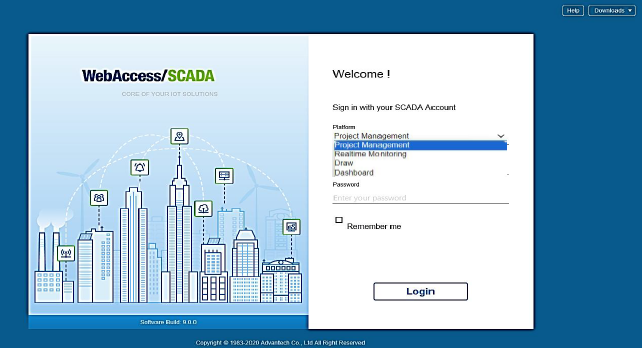
\includegraphics[width=0.85\linewidth]{figures/Exp9_Figure_1.png}
            \captionof{figure}{WebAccess landing page}
            \label{fig:exp9-webaccess}
          \end{boxedfigure}

    \item Create a new project: enter a \textbf{Project Name} and \textbf{Project Description}, and set the \textbf{Project Node IP Address} (use \texttt{127.0.0.1} for a local machine, or the PC's hostname) as in Figure~\ref{fig:exp9-projectcreate}.
          \begin{boxedfigure}
            \centering
            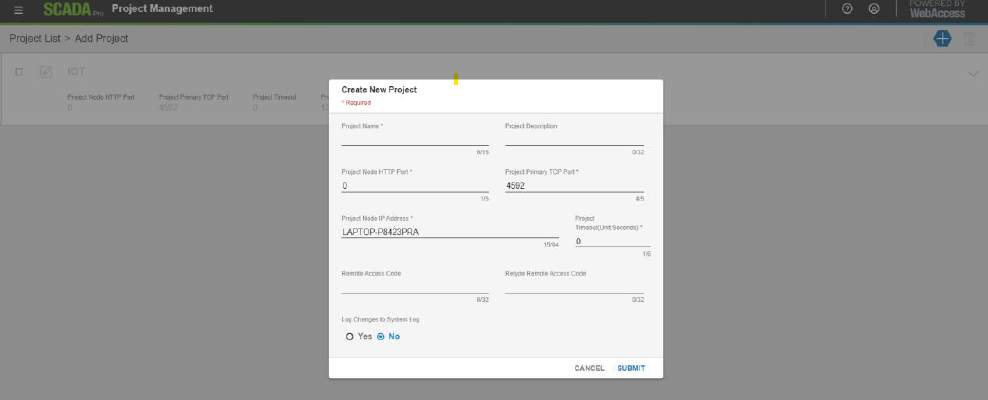
\includegraphics[width=\linewidth]{figures/Exp9_Figure_2.png}
            \captionof{figure}{New project creation.}
            \label{fig:exp9-projectcreate}
          \end{boxedfigure}

    \item Leave the \textbf{Primary TCP Port} (default \texttt{4592}) and \textbf{HTTP Port} (default \texttt{80}) at their defaults unless your network/firewall requires otherwise, then click \textbf{Submit}.
    \item Select the Project Node in the tree structure, click \textbf{+}, and choose \textbf{New Node} to create the SCADA Node. Fill in the Primary Node Name, Primary/Secondary TCP Port, Node Timeout, and SCADA Node IP Address. Refer to Figure~\ref{fig:exp9-scadanode}.
          \begin{boxedfigure}
            \centering
            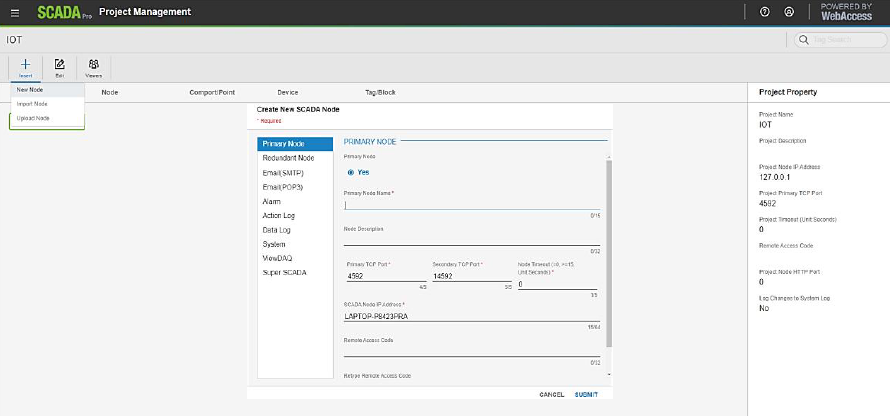
\includegraphics[width=\linewidth]{figures/Exp9_Figure_3.png}
            \captionof{figure}{New project creation.}
            \label{fig:exp9-scadanode}
          \end{boxedfigure}
    \item Start the Kernel on the SCADA Node (\textbf{Start Kernel} from the SCADA Node menu) and confirm it is running by hovering over the WebAccess/SCADA icon, which should report the running project and node name.
  \end{enumerate}
  \newpage

  \textbf{Activity 2 --- Configure a communication port and add a device}\vspace{2pt}

  \textit{Objective: create the physical/virtual link (Comport) between the SCADA node and the PLC, and add the PLC as a device on that port.}

  \begin{enumerate}
    \item Under the SCADA Node, add a new \textbf{Comport}. Select the interface type appropriate to your connection:
          \begin{itemize}
            \item \textbf{Serial} --- an RS232/RS422/RS485 port (COM1, COM2, \ldots) on the SCADA node PC.
            \item \textbf{TCP/IP} --- the most common choice for PLCs and IoT devices; WebAccess/SCADA searches all TCP/IP network cards regardless of the assigned Comport number (Figure~\ref{fig:exp9-comport}).
                  \begin{boxedfigure}
                    \centering
                    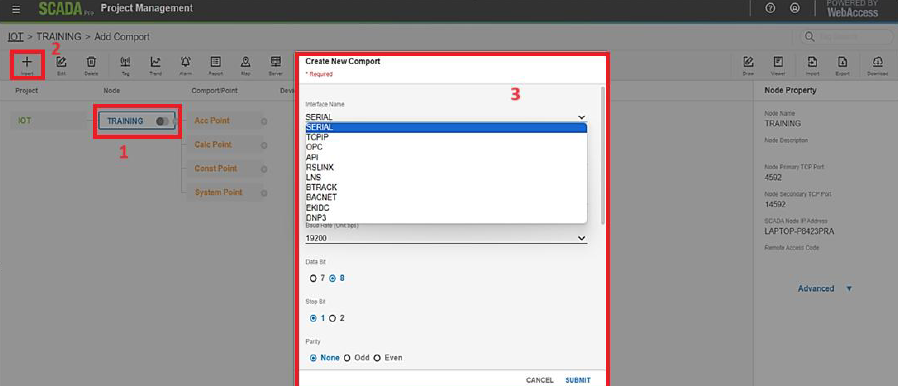
\includegraphics[width=\linewidth]{figures/Exp9_Figure_4.png}
                    \captionof{figure}{COMPort selection.}
                    \label{fig:exp9-comport}
                  \end{boxedfigure}
            \item \textbf{OPC} --- via an OPC Server, for virtual/software-based links.
          \end{itemize}
    \item Configure the port: Port Number, Scan Time (e.g.\ \texttt{1000\,ms}), and Auto-recover Time.
    \item Under the configured Comport, add a new \textbf{Device}, selecting the correct Device Type/Driver for your hardware (e.g.\ Siemens S7-1200, Modbus TCP, Allen-Bradley) as in Figure~\ref{fig:exp9-S71200Config}.
    \item Enter the device's communication parameters (IP address, station ID, or baud rate for serial links) and save.
          \begin{boxedfigure}
            \centering
            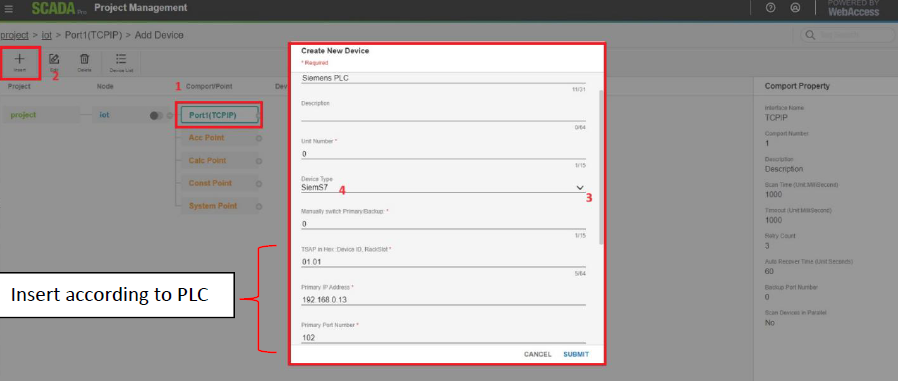
\includegraphics[width=0.9\linewidth]{figures/Exp9_Figure_5.png}
            \captionof{figure}{Siemens S7-1200 device configuration.}
            \label{fig:exp9-S71200Config}
          \end{boxedfigure}
  \end{enumerate}
  \newpage

  \textbf{Activity 3 --- Create IO Tags}\vspace{2pt}

  \textit{Objective: choose a subset of the available sensors and create IO Tags that map them into SCADA.}

  \begin{enumerate}
    \item From Table~\ref{tab:exp9scada-sensors}, select \textbf{at least five} sensors/signals to bring into your SCADA project. Your selection must include:
          \begin{itemize}
            \item all three digital control inputs (Start, Stop, Emergency stop),
            \item at least one analog process value (e.g.\ Temperature, Humidity, Vibration, or Distance), and
            \item at least one production/OEE value (Availability, Good part, Defect part, or Total output).
          \end{itemize}
          This selection is the basis for the dashboard you will build later in this experiment, so choose sensors that will make a meaningful, connected display (for example, a temperature reading alongside Good/Defect part counts tells a more coherent story than five unrelated signals).
    \item For each selected signal, take its address from Table~\ref{tab:exp9scada-sensors} (S7-1200 direct or OPC, depending on which Comport/Device you configured in Activity 2) and convert it to the equivalent WebAccess tag addressing using Table~\ref{tab:exp9scada-addrmap} as a reference.
    \item Under the Device, click the tag icon and \textbf{Insert} a new tag for each signal. Fill in the Tag Type, Tag Name, Address, Start Bit, Conversion Code, and Length fields to match your addressing, and set \textbf{Log Data} to \textbf{Yes} for every tag --- this is required for the tag's history to reach the dashboard you build later in this experiment.
    \item Save your tags, then verify each one updates correctly by forcing the corresponding input/output in the PLC and observing the tag's live value in WebAccess.
  \end{enumerate}
  \vspace*{1.5em}

  \textbf{Activity 4 --- Create Internal Tags}\vspace{2pt}

  \textit{Objective: create at least one Constant Tag and one Calculation Tag.}

  \begin{enumerate}
    \item Under \textbf{Const Point} on the SCADA Node, insert a new Constant Tag (analog type, \texttt{ConAna}, or discrete type, \texttt{ConDis}) --- for example, a user-adjustable setpoint value.
    \item Under \textbf{Calc Point} on the SCADA Node, insert a new Calculation Tag. Choose an analog or discrete result type, then write a mathematical/logical expression referencing one or more of your IO Tags (tags are referenced in the formula by their single-letter designations; the expression is limited to 80 characters).
    \item Save and verify that the Calculation Tag's value updates correctly as its input tag(s) change.
  \end{enumerate}
  \vspace*{1.5em}

  \textbf{Activity 5 --- Configure a basic alarm}\vspace{2pt}

  \textit{Objective: enable alarming on at least one analog tag and one discrete tag.}

  \begin{enumerate}
    \item Open the configuration for one of your Analog IO Tags and enable a non-zero alarm priority. Analog tags support High-High, High, Low, Low-Low, Deviation, and Rate-of-Change alarms --- choose whichever is appropriate to the signal you selected.
    \item Open the configuration for one of your Discrete IO Tags and enable state alarming (e.g.\ alarm when the E-stop input becomes active).
    \item Trigger each alarm condition on the PLC side and confirm that the alarm appears correctly in WebAccess.
  \end{enumerate}
  \vspace*{1.5em}

  \textbf{Activity 6 --- Enable ODBC data logging}\vspace{2pt}

  \textit{Objective: configure the SCADA Node to log tag history out to the external database, so it is available to the dashboard you build next.}

  \begin{enumerate}
    \item Select your SCADA Node, then open \textbf{Edit Node} $\to$ \textbf{Data Log}.
    \item Set \textbf{Data Log To ODBC} to \textbf{Yes}.
    \item Set the \textbf{Data Log Interval} (in seconds or minutes) to a value appropriate for your selected sensors --- a value of \texttt{0} logs by deadband instead of on a fixed schedule.
    \item Confirm the \textbf{Data Log Starting Year} matches the current year, then click \textbf{Submit}.
    \item Confirm with your instructor that the ODBC connection target (PostgreSQL host, database, and schema) is already configured on this machine --- this experiment assumes that connection exists; setting it up is outside the scope of this lab.
  \end{enumerate}
  \vspace*{1.5em}

  \textbf{Activity 7 --- Connect the Dashboard to its data source}\vspace{2pt}

  \textit{Objective: open WISE-IoTSuite/Dashboard and point it at the PostgreSQL database your SCADA node is logging to.}

  \begin{enumerate}
    \item Return to the WebAccess/SCADA landing page and, from the \textbf{Platform} drop-down, select \textbf{Dashboard} instead of Project Management. Sign in with the same SCADA account, then choose your project.
          \begin{boxedfigure}
            \centering
            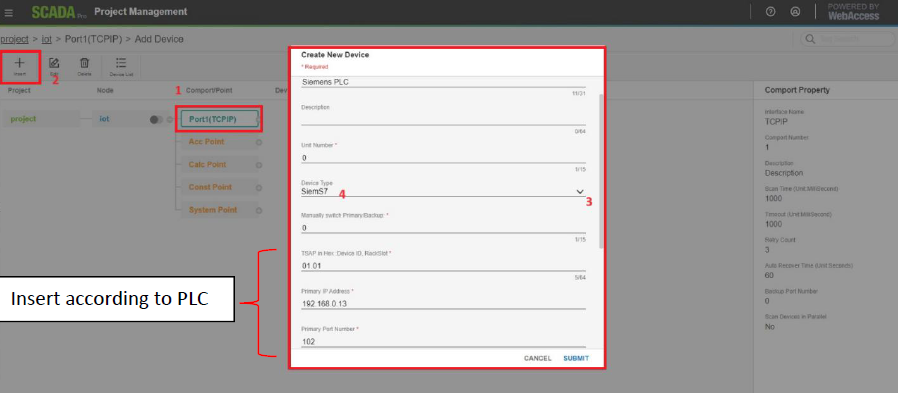
\includegraphics[width=\linewidth]{figures/Exp9_Figure_6.png}
            \captionof{figure}{Dashboard login via the Platform dropdown.}
            \label{fig:exp9-dashboardlogin}
          \end{boxedfigure}
    \item On the Dashboard home page, open the gear/\textbf{Configuration} icon on the left-hand toolbar, then select \textbf{Data Sources}.
    \item Check whether a \textbf{PostgreSQL} data source already exists for your instructor's ODBC target. If not, click \textbf{Add data source}, choose \textbf{PostgreSQL} from the SQL section, and enter the connection details provided by your instructor (Host, Database, Schema, User); leave \textbf{SSL Mode} as \textbf{disable} unless told otherwise.
          \begin{boxedfigure}
            \centering
            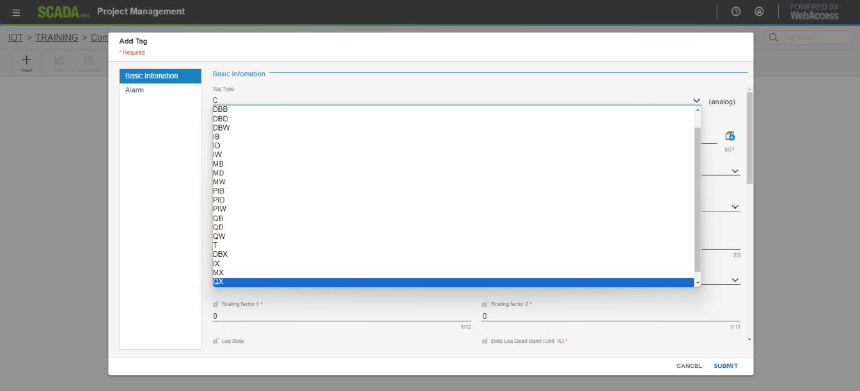
\includegraphics[width=\linewidth]{figures/Exp9_Figure_7.png}
            \captionof{figure}{Adding a PostgreSQL data source.}
            \label{fig:exp9-postgresdatasource}
          \end{boxedfigure}
    \item Click \textbf{Save \& Test}. If the test fails, double-check the host/port and that your SCADA Node's ODBC logging (Activity 6) has actually written at least one value --- an empty log table is a common reason a working connection still looks ``wrong'' when you first query it.
  \end{enumerate}
  \vspace*{1.5em}

  \textbf{Activity 8 --- Build a dashboard for your selected sensors}\vspace{2pt}

  \textit{Objective: create a dashboard with panels displaying the sensors you selected in Activity 3.}

  \begin{enumerate}
    \item From the Dashboard home page, create a \textbf{new Dashboard} and give it a descriptive name.
    \item Add at least \textbf{three} panels, using at least \textbf{two different panel types} from the following:
          \begin{itemize}
            \item \textbf{Singlestat} --- a single current value, suited to a live reading (e.g.\ Temperature, Humidity).
            \item \textbf{Graph} --- a time-series trend, suited to a value that changes meaningfully over time (e.g.\ Vibration, a running production count).
            \item \textbf{Control Panel} --- suited to showing/annotating a discrete state (e.g.\ Start/Stop/E-stop status).
            \item \textbf{Advanced Datatable} --- suited to displaying several related values together in one table (e.g.\ Good part / Defect part / Total output side by side).
          \end{itemize}
    \item For each panel, open its \textbf{Query} settings, select your PostgreSQL data source, and choose the \texttt{data log} table. Pick the tag(s) you created in Activity 3 by name, and set an appropriate time range (for a Graph panel) or leave it as the latest value (for a Singlestat).
          \begin{boxedfigure}
            \centering
            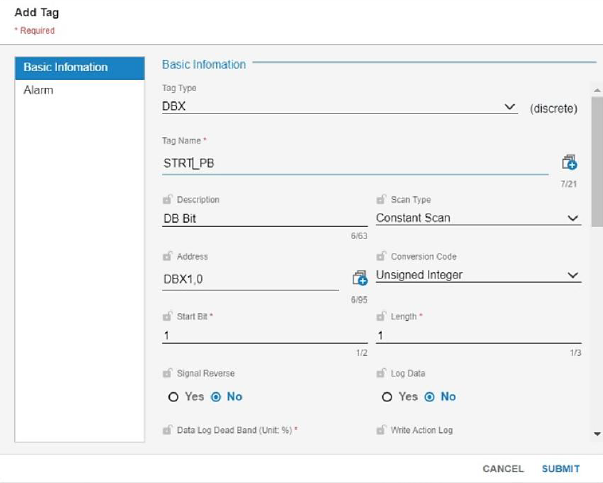
\includegraphics[width=\linewidth]{figures/Exp9_Figure_8.png}
            \captionof{figure}{Panel query configuration: data source, table, and tag selection.}
            \label{fig:exp9-panelquery}
          \end{boxedfigure}
    \item Arrange and resize your panels into a coherent layout, then \textbf{save} the dashboard.
    \item With the PLC running, confirm that each panel updates: force a change on the PLC side (e.g.\ press Start, or change an analog input) and verify the corresponding panel reflects it within your configured Data Log Interval.
  \end{enumerate}

\end{procedure}

\begin{reportq}
  \begin{enumerate}
    \item List the Project Node and SCADA Node settings you used (IP address, ports, node names), and explain the role each plays in the system.
    \item Present your Comport and Device configuration, including which interface type (Serial/TCP-IP/OPC) you selected and why it was appropriate for your hardware.
    \item State which sensors/signals you selected from Table~\ref{tab:exp9scada-sensors} and why --- what did you intend to show on your dashboard, and how did that shape your choice?
    \item Tabulate the IO Tags you created: PLC address, WebAccess address, tag type, and a description of what each represents.
    \item Present your Constant Tag and Calculation Tag configurations, including the expression used for the Calculation Tag and what it computes.
    \item Describe the alarm(s) you configured and demonstrate (with a screenshot or description of your test) that each triggers correctly.
    \item State your Data Log to ODBC settings (interval, starting year) and explain, in your own words, the full path a value takes from the PLC to the point where it becomes available to the Dashboard.
    \item Include a screenshot of your finished dashboard, and for each panel state which tag(s) it displays and why you chose that panel type (Singlestat/Graph/Control Panel/Advanced Datatable) for that particular sensor.
    \item Describe one problem you encountered while connecting the Dashboard to its data source or building a panel, and how you resolved it.
    \item Discuss one advantage of WebAccess/SCADA's 100\% web-based architecture compared to a traditional desktop-client SCADA system.
  \end{enumerate}
\end{reportq}

\begin{labsection}{References}{}
  \begin{itemize}
    \item MTA SkillLab Sdn Bhd, \textit{i-Factory Training Manual --- IIoT System Development Level 1}, Module 3: Project Creation in SCADA (\texttt{Scada\_OPC.pdf}).
    \item MTA SkillLab Sdn Bhd, \textit{i-Factory Training Manual --- IIoT System Development Level 1}, Module 4: Dashboard Viewing and Analysis (\texttt{Dashboard\_IoT\_WIISE.pdf}).
    \item MTA SkillLab Sdn Bhd, \textit{Parameter in OEE Monitoring System} --- sensor/tag address reference for the S7-1200 trainer, direct and OPC addressing (\texttt{OEEE\_Monitoring\_System\_Param.pdf}).
    \item MTA SkillLab Sdn Bhd, \textit{Quick Guide: Configure a Project} --- condensed step summary, Steps 1--7 (\texttt{Simplified\_LabSheet.pdf}).
    \item Advantech WebAccess/SCADA product documentation: \url{https://www.advantech.com/en/support/details/installation?id=1-MS9MJV}
  \end{itemize}
\end{labsection}